% !TEX root=report.tex
\section{Features}

Couchsurfing.org provided us with an anonymized copy of their databases giving us access to a variety of interesting properties of their users (surfers/hosts). 
Broadly speaking we use features describing personal information like age, gender, languages spoken, countries lived in, countries traveled to, etc., their interests (extracted from the free form text on their profiles, for more information see Section TODO), and their status and activity on Couchsurfing.org which includes e.g. the number of references, the number of friends, or the response rate in the internal messaging system.

% TODO: to illustrate this a figure might be helpful
We developed a general approach how we deal with a wide variety of features. For each feature (e.g. age) we look at the value distribution in the training set and build a histogram where the boundaries between the bins are based on the inverse distribution function of the values (to obtain a roughly uniform distribution over the chosen bins). Using this mapping from value to bin we can binarize each feature by mapping it to a binary vector (e.g. $age=27$ maps to bin \#4 or the vector $b=[0,0,0,1,0,\dots]^T$). Since our feature $\Phi(s,h)$ is based on both the surfer $s$ and the host $h$ we include this binary vector for both of them as well as the outer product between the two, $b_s b_h^T$, in our final feature. The outer product also captures all combinations of the binned features. For example, we can capture that hosts between 21 and 25 years old prefer having surfers of the same age stay with them while hosts age 60 and above don't have any particular preferences regarding the age. Other example inlude capturing affinities between genders, countries, spoken languages, certain interest groups, etc.


%sometimes additional manually designed features (e.g. how many languages sb speaks or how many languages they have in common) WE DONT DO THAT ATM


\subsection{User interests}
\todo{add some more information about interest extraction + interest graph + clustering + interest feature here}
Interest graph: the compatibility strength between surfer and host is determined by $num_overlapping_interest(host, surfer)$ through some type of decaying activation propagation.  This will be based on the "Taste Fabric" paper and the "Semantic Recommendation" paper.  This method assumes homophily and that interests are the strongest attractors between people (doesn't take into account demographics etc.).  This method is reversible.

\begin{figure}[ht]
\centering
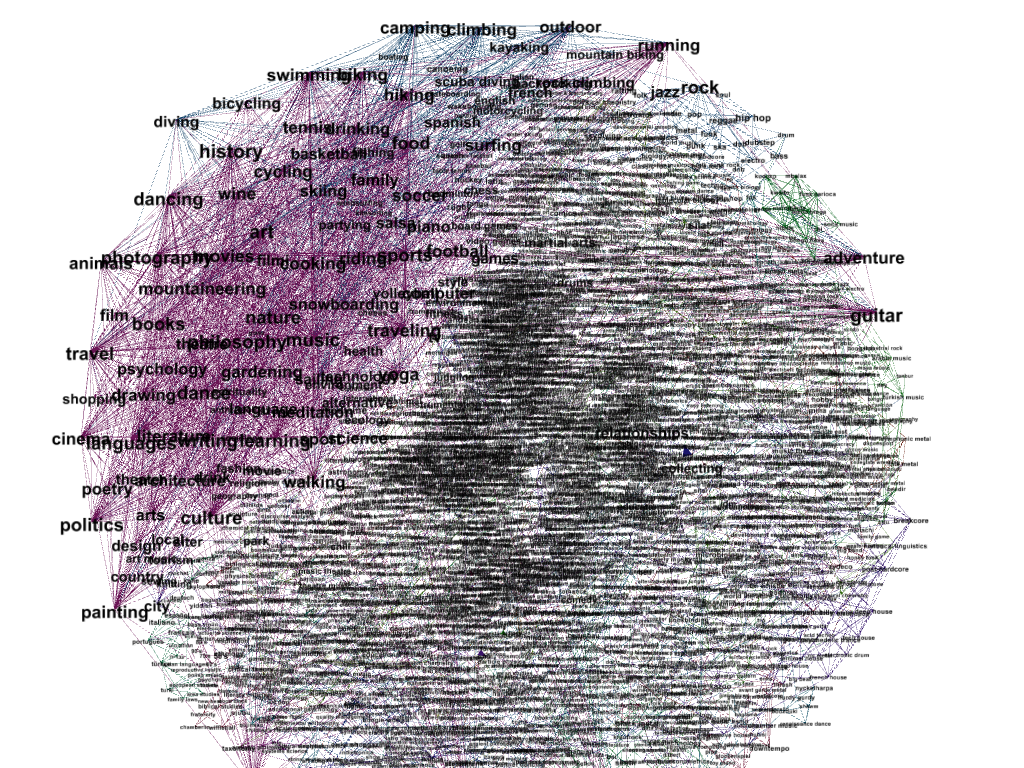
\includegraphics[width=1\linewidth]{figures/interest_graph.png}
\caption{Interest graph.}
\label{fig:interest_graph}
\end{figure}
